\documentclass[11pt,a4paper]{article}

\usepackage{graphicx}
\usepackage{caption}
\usepackage{fancyhdr}
\usepackage{textcomp}
\usepackage{float}
\usepackage[headheight=10pt]{geometry}
\usepackage[acronyms,nomain,nonumberlist]{glossaries}

\usepackage{listings}
\lstset{
	tabsize=2,
	frame=single,
	columns=flexible,
	breaklines=true
}

%\usepackage[backend=biber,sorting=ynt,style=ieee]{biblatex}
%\bibliography{referenties.bib}

\pagestyle{fancy}

\newcommand\blankpage{%
	\newpage
	\null
	\thispagestyle{empty}%
	\newpage}

\renewcommand{\contentsname}{Inhoudstabel}
\renewcommand{\listfigurename}{Lijst met figuren}
\renewcommand{\listtablename}{Lijst met tabellen}
\renewcommand{\headrulewidth}{0pt}

\loadglsentries{acronyms}
\makeglossaries

\title{\vfill Ingebedde systemen: project - controller voor servomotoren}
\author{Francis Begyn en Heleen Cauwels}
\date{2017 \vfill}

\begin{document}
	
	\begin{titlepage}
		\maketitle
		\centering Begeleider: Dimitri Van Cauwelaert
		\thispagestyle{fancy}
		\fancyhf{}
		\rhead{\includegraphics*{ugent}}
		\cfoot{\includegraphics*{faculteit}}
	\end{titlepage}
	
	\renewcommand{\headheight}{10pt}
	\fancyhf{}
	\cfoot{\thepage}
	\addtocounter{page}{+1}
	
	\addcontentsline{toc}{section}{Inhoudstabel}
	\tableofcontents
	\newpage
	
	\addcontentsline{toc}{section}{Lijst met figuren}
	\listoffigures
	\newpage
	
	%\addcontentsline{toc}{section}{Lijst met tabellen}
	%\listoftables
	%\newpage
	
	\addcontentsline{toc}{section}{Lijst met afkortingen}
	\printglossary[type=\acronymtype,title={Lijst met afkortingen}]
	\newpage
	
	\addcontentsline{toc}{section}{Inleiding}
	\section*{Inleiding}
	De opdracht is het maken van een controller voor een servomotor in VHDL en een testbench om deze te kunnen uittesten. Hier is het ook belangrijk om rekening te houden met de vereisten van de klant en indien nodig het apparaat aan te passen.\\
Een servomotor is een motor die door middel van \gls{pwm} aangestuurd kan worden naar een gewenste positie en deze in normale operatie zal behouden. De snelheid waarmee deze behouden wordt, is afhankelijk van de kloksnelheid die aan de controller meegeven wordt.
	
	\newpage
	\section{Vereisten en afspraken van de controller}
	De controller moet in staat om een servomotor over 180\textdegree \space aan te sturen met \gls{pwm} signalen tussen 1,25 ms en 1,75 ms. De reset verloopt synchroon met de klok, dit is om te verhinderen dat het \gls{pwm} signaal vervormt zou worden door de slechte timing van een reset. In het geval van asynchrone reset, zou het  signaal onbedoeld langer kunnen worden dan de maximum pulsduur (1,75 ms).\\
\\
De controller werkt met een klok van 50 Hz en een servoklok van 510 kHz. Hiermee rekening houdende blijkt dat de minimum pulsduur van 1,25 ms overeen komt met 637,5 servoklok ticks, het midden van 1.5 ms komt overeen met 765 servoklok ticks en de maximum pulsduur van 1,75 ms komt overeen met 892,5 servoklok ticks. In \gls{vhdl} wordt gewerkt met unsigned variabelen, dus 637,5 en 892,5 worden afgerond naar respectievelijk 637 en 892.\\
\\
Elke servocontroller heeft een adres. Als er een positie gestuurd wordt die vooraf gegaan wordt door het correcte adres, dan moet de controller deze instructie uitvoeren. Indien een ander adres vermeld wordt dan moet de controller de opdracht negeren.\\
Ook is er een \textit{broadcast} adres waar alle controllers  naar moeten luisteren, namelijk 255. Als een signaal uitgestuurd wordt met het \textit{broadcast} adres dan moeten alle aangesloten controllers hetzelfde \gls{pwm} signaal generen.\\
\\
Onder normale operatie zal de controller de positie behouden, maar als er iets fout loopt zal de controller de servomotor terugzetten naar zijn neutrale positie. De neutrale positie wordt hier gedefinieerd als op 90\textdegree, en komt overeen met een pulsduur van 1,5ms. De controller keert ook naar deze neutrale positie terug indien een reset opgeroepen wordt.\\
\\
Het Done signaal werk met \textit{tri-state logic}, dit betekend dat het op een bus aangesloten kan worden. Hierdoor kunnen meerdere controllers gebruik maken van \'{e}\'{e}nzelfde bus, waardoor er bespaard kan worden op het aantal kabels dat nodig is.\\
\\
Als de aansturende microcontroller tijdens het aansturen van de controller beslist om een taak van hogere prioriteit uit te voeren, moet de controller dit kunnen afhandelen en naar de neutrale positie gaan.\\

	
	\newpage
	\section{Verslag code}
	\subsection{Entity}
De entity van de servocontroller beschrijft de poortmapping. De servoctontroller neemt clk (clock), rst (reset), sclk (servoclock), set en data als inputs. De servocontroller zal het done signaal en het aanstuursignaal (pwm) als uitput genereren. Er is voor gekozen om een generische variabele address toe te voegen, zodat de code kan herbruikt worden voor verschillende adressen.
\lstinputlisting{servocontroller_entity.vhd}
	\subsection{Architecture}
In het begin van de architectuur defini\"{e}ren we de benodigde signalen. Op basis van de hulpsignalen cnt en pwmi kunnen we een PWM signaal generen (zie gen\_pwm). Daarna worden de nodige types en signalen aangemaakt om een \gls{fsm} te kunnen gebruiken. Eerst worden de verschillende staten gedefinieerd waarna de signalen voor het bijhouden van de staat (currentState en nextState) ook aangemaakt worden.

\lstinputlisting[firstline=1,lastline=14]{servocontroller_arch.vhd}
State\_trans beschrijft de transities tussen verschillende staten. De transities worden beschreven in volgend flowchart.
\begin{figure}[h]
	\centering
	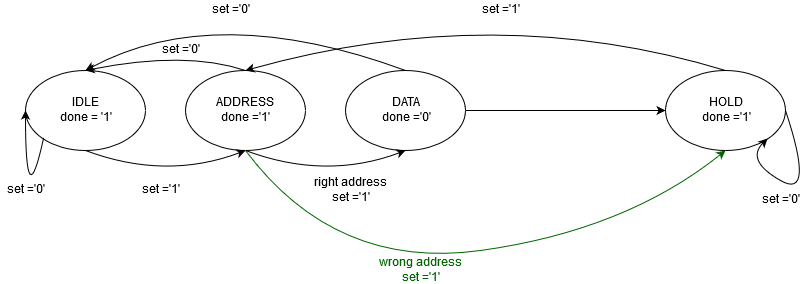
\includegraphics[width=\linewidth]{servocontrol.png}
	\caption{Transitiediagram voor de \gls{fsm} van de servocontroller}
\end{figure}\\
 Voordat de controller het \gls{pwm} signaal aanmaakt, moet er gecontroleerd worden of het doorgestuurde adres enerzijds het \textit{broadcast} adres is, of anderzijds het adres is van de servomotor. Anders mag de controller zijn output niet aanpassen. Indien het set-signaal onderbroken wordt, voordat er een nieuwe positie is doorgestuurd, moet de controller naar de neutrale positie (idle) gaan.

\lstinputlisting[firstline=17,lastline=49]{servocontroller_arch.vhd}
Transition is het proces dat de overgangen van de staten dicteert. Hier wordt er ook voor gezorgd dat bij een reset de controller altijd terug gaat naar neutrale (idle) positie, ongeacht de status van de andere signalen.

\lstinputlisting[firstline=51,lastline=58]{servocontroller_arch.vhd}
Set\_output dicteert hoe het \textit{done} signaal zich gedraagt in elke staat. In deze setup heeft done een \textit{tri-state logic}. Het \gls{pwm} signaal wordt hier niet gedefinieerd omdat er een one-line process gebruikt wordt om dit aan de uitgang te koppelen (zie gen\_pwm).

\lstinputlisting[firstline=60,lastline=82]{servocontroller_arch.vhd}
Pwm\_data is het proces dat de berekeningen en lengte van de puls bepaalt. Op basis van de servoklok wordt berekend welke waarden nodig zijn om de gewenste pulsen te bekomen. In commentaar zijn de berekende waarden voor een servoklok van 510kHz te vinden. Indien de servoklok aangepast wordt, moet deze code aangepast worden zodat de juiste waarden gebruikt worden.

\lstinputlisting[firstline=84,lastline=99]{servocontroller_arch.vhd}
Gen\_pwm is het proces dat de eigenlijke puls genereert. Het aantal servoklok ticks wordt bijgehouden en vergeleken met de benodigde aantallen die in pwm\_data bepaald zijn. Cnt moet gereset worden bij elke klok tick (50 Hz).\\
Nadien wordt met een one-line process het pwm signaal aan de output gekoppeld. \label{one-liner}

\lstinputlisting[firstline=101,lastline=114]{servocontroller_arch.vhd}
	\subsection{Testbench}

De testbench is verantwoordelijk om de geschreven architecture uit te testen. De vereiste van de testbench is dat deze een klok en servoklok genereert, de servocontroller uittest in stappen van 32, de positie van de servomotor opvraagt en controleert. De servoklok mag niet gebruikt worden om het PWM signaal te controleren.
	
	\newpage
	\section*{Conclusie}
	Er werd een servocontroller ontworpen in \gls{vhdl}. Deze controller moest voldoen aan verschillende specificaties, zowel specificaties uit de oorspronkelijke opdracht, als verdere specificaties besproken met de begeleider. Er werd ook een testbench voor de servocontroller geschreven die bovenstaande specificaties test.\\
\\
\noindent
Door de testbench een beetje aan te passen, kan men aan tonen dat de controller ook in staat is om zelf met stappen van 2 nog heel goed te werken. Men kan de controller dus ook gebruiken om een grotere precisie te bekomen dan de vereisten oplegden.
	
	%\addcontentsline{toc}{section}{Referenties}
	%\printbibliography[title={Referenties}]
	
	\blankpage
\end{document}